%%%%%%%%%%%%%%%%%%%%%%%%%%%%%%%%%%%%%%%%%
% Short Sectioned Assignment LaTeX Template Version 1.0 (5/5/12)
% This template has been downloaded from: http://www.LaTeXTemplates.com
% Original author:  Frits Wenneker (http://www.howtotex.com)
% License: CC BY-NC-SA 3.0 (http://creativecommons.org/licenses/by-nc-sa/3.0/)
%%%%%%%%%%%%%%%%%%%%%%%%%%%%%%%%%%%%%%%%%

%----------------------------------------------------------------------------------------
%	PACKAGES AND OTHER DOCUMENT CONFIGURATIONS
%----------------------------------------------------------------------------------------

\documentclass[paper=a4, fontsize=11pt]{scrartcl} % A4 paper and 11pt font size

% ---- Entrada y salida de texto -----

\usepackage[T1]{fontenc} % Use 8-bit encoding that has 256 glyphs
\usepackage[utf8]{inputenc}
%\usepackage{fourier} % Use the Adobe Utopia font for the document - comment this line to return to the LaTeX default

% ---- Idioma --------

\usepackage[spanish, es-tabla]{babel} % Selecciona el español para palabras introducidas automáticamente, p.ej. "septiembre" en la fecha y especifica que se use la palabra Tabla en vez de Cuadro

% ---- Otros paquetes ----

\usepackage{url} % ,href} %para incluir URLs e hipervínculos dentro del texto (aunque hay que instalar href)
\usepackage{hyperref}
\hypersetup{
	colorlinks=true,
	linkcolor=black,
	urlcolor=black,
	citecolor=black,
}
\usepackage{amsmath,amsfonts,amsthm} % Math packages
%\usepackage{graphics,graphicx, floatrow} %para incluir imágenes y notas en las imágenes
\usepackage{graphics,graphicx, float} %para incluir imágenes y colocarlas

% Para hacer tablas comlejas
%\usepackage{multirow}
%\usepackage{threeparttable}

%\usepackage{sectsty} % Allows customizing section commands
%\allsectionsfont{\centering \normalfont\scshape} % Make all sections centered, the default font and small caps

\usepackage{fancyhdr} % Custom headers and footers
\pagestyle{fancyplain} % Makes all pages in the document conform to the custom headers and footers
\fancyhead{} % No page header - if you want one, create it in the same way as the footers below
\fancyfoot[L]{} % Empty left footer
\fancyfoot[C]{} % Empty center footer
\fancyfoot[R]{\thepage} % Page numbering for right footer
\renewcommand{\headrulewidth}{0pt} % Remove header underlines
\renewcommand{\footrulewidth}{0pt} % Remove footer underlines
\setlength{\headheight}{13.6pt} % Customize the height of the header

\numberwithin{equation}{section} % Number equations within sections (i.e. 1.1, 1.2, 2.1, 2.2 instead of 1, 2, 3, 4)
\numberwithin{figure}{section} % Number figures within sections (i.e. 1.1, 1.2, 2.1, 2.2 instead of 1, 2, 3, 4)
\numberwithin{table}{section} % Number tables within sections (i.e. 1.1, 1.2, 2.1, 2.2 instead of 1, 2, 3, 4)

\setlength\parindent{0pt} % Removes all indentation from paragraphs - comment this line for an assignment with lots of text

\newcommand{\horrule}[1]{\rule{\linewidth}{#1}} % Create horizontal rule command with 1 argument of height
\usepackage{booktabs}

\usepackage{listings}
\lstdefinelanguage
[x64]{Assembler}     % add a "x64" dialect of Assembler
[x86masm]{Assembler} % based on the "x86masm" dialect
{morekeywords={CDQE,CQO,CMPSQ,CMPXCHG16B,JRCXZ,LODSQ,MOVSXD, %
		POPFQ,PUSHFQ,SCASQ,STOSQ,IRETQ,RDTSCP,SWAPGS, %
		rax,rdx,rcx,rbx,rsi,rdi,rsp,rbp, %
		r8,r8d,r8w,r8b,r9,r9d,r9w,r9b, %
		r10,r10d,r10w,r10b,r11,r11d,r11w,r11b, %
		r12,r12d,r12w,r12b,r13,r13d,r13w,r13b, %
		r14,r14d,r14w,r14b,r15,r15d,r15w,r15b}} % etc.
\usepackage{color}
\usepackage{xcolor}
\lstdefinestyle{customc}{
	belowcaptionskip=1\baselineskip,
	breaklines=true,
	frame=L,
	xleftmargin=\parindent,
	language=C,
	showstringspaces=false,
	basicstyle=\footnotesize\ttfamily,
	keywordstyle=\bfseries\color{green!40!black},
	commentstyle=\itshape\color{purple!40!black},
	identifierstyle=\color{blue},
	stringstyle=\color{orange},
}

\lstset{escapechar=@,style=customc}
\usepackage{url}

\title{	
	\normalfont \normalsize
	\begin{figure}[htb]
		\centering
		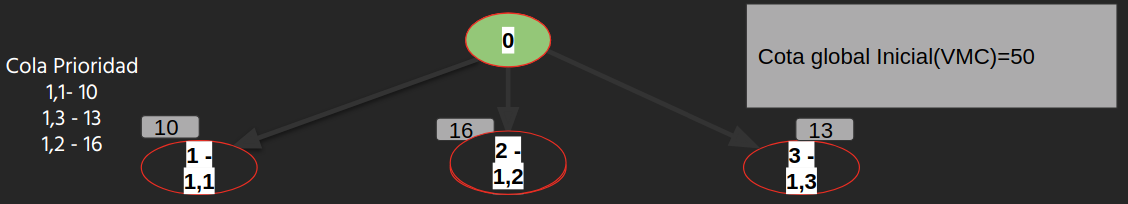
\includegraphics[width=0.3\textwidth]{./imagenes/1}
	\end{figure}
	\textsc{\textbf{Algoritmica} \\ Grado en Ingeniería Informática \\ 
	Curso 2018-2019} \\ [25pt] 
	\begin{figure}[htb]
		\centering
		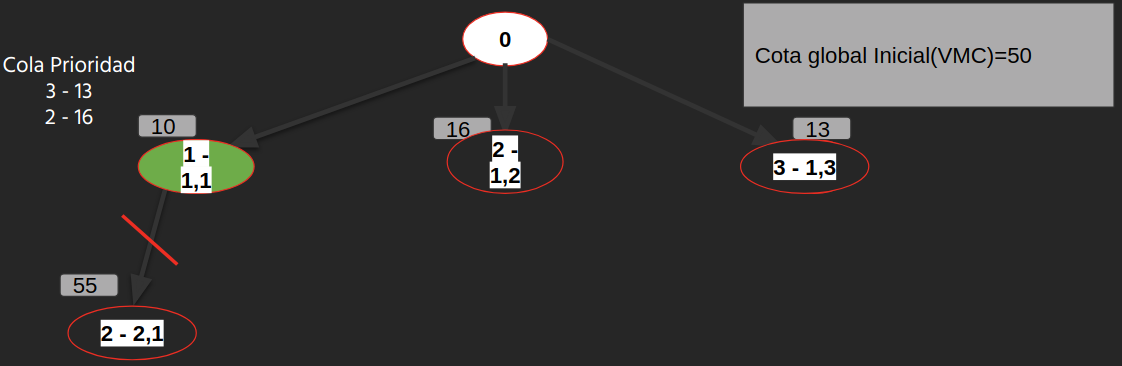
\includegraphics[width=0.15\textwidth]{./imagenes/2}
	\end{figure}
	\horrule{0.5pt} \\[0.4cm]
	\huge Ejercicio Propuesto. \\
	\huge 8-Reinas
	\\ 
	\horrule{2pt} \\[0.5cm] 
}
\author{Félix Ramírez García  \\
\href{mailto:felixramirezgarcia@correo.ugr.es}{felixramirezgarcia@correo.ugr.es}}
\date{\normalsize\today} 

%----------------------------------------------------------------------------------------
% DOCUMENTO
%----------------------------------------------------------------------------------------

\begin{document}
	
	\maketitle % Muestra el Título
	
	\newpage %inserta un salto de página
	
	\tableofcontents % para generar el índice de contenidos
	
	\listoffigures % para generar índice de imágenes.
	
	\listoftables % para generar índice de tablas.
	
	\newpage
	
	%-----------------------------------------------------------------------
	%							Introduccion
	%----------------------------------------------------------------------	
	\section[Introducción]{Introducción}
	
	El problema de las ocho reinas es un pasatiempo que consiste en poner ocho reinas en el tablero de ajedrez sin que se amenacen. En el juego del ajedrez la reina amenaza a aquellas piezas que se encuentren en su misma fila, columna o diagonal. Para resolver este problema emplearemos un esquema vuelta atrás. \\
	
	El problema de las ocho reinas se puede plantear de modo general como problema de las n reinas. El problema consistiría en colocar n reinas en un tablero de ajedrez de nxn de tal manera que ninguna de las reinas quede atacando a otras.
	
	%-----------------------------------------------------------------------
	%							Solucion fuerza bruta
	%----------------------------------------------------------------------	
	\section[Solución fuerza bruta]{Solución fuerza bruta}
	
	El método de la fuerza bruta aplicado al problema de las reinas consistiría en calcular todas las formas posibles de colocar las ocho piezas en el tablero, y para cada una de ellas comprobar si se trata de una posición legal, es decir, no hemos colocado más de una reina en la misma casilla, y que las reinas no se atacan entre sí (no hay dos reinas situadas en la misma fila, columna, o diagonal). De esta manera, la primera pieza la podríamos colocar en cualquiera de las 64 casillas; la segunda, también se podría colocar en cualquiera de las 64 casillas (y después ya comprobaremos si las hemos colocado en la misma), con lo que tendríamos 64x64 posibilidades; con la tercera pieza tendríamos 64x64x64 posibilidades; y cuando coloquemos la última, tendríamos 64x64x64x64x64x64x64x64 posibilidades, que nos da el astronómico número de 281.474.976.710.656 posiciones a examinar, algo que está fuera del alcance de la mayoría de los ordenadores de hoy en día.\\
	
	El código usado para solventar este problema es el que se muestra a continuación: \\
	
	\lstset{language=C}
	\begin{lstlisting}[frame=single]
#include <stdio.h>
#include <stdlib.h>
#include <time.h> 
#include <vector>
#include <iostream>
#include <ctime>
#include <cstdlib>
#include <climits>
#include <cassert>
#include <string>
#include <fstream>
#include <chrono>
#define MAX_N (30)

using namespace std;
using namespace std::chrono;

high_resolution_clock::time_point tantes, tdespues;
duration<double> transcurrido;

int tablero[MAX_N] ;
int total = 0 ;

#define abs(n) ((n)<(0)?(-(n)):(n))

void comprobar(int tablero[MAX_N], int n)
{
	int col[MAX_N] ;
	int i, j ;
	for (i=n-1; i>=0; i--) {
		col[i] = tablero[i] ;
		for (j=i+1; j<n; j++) {
			if (col[i] <= col[j]) 
		col[j]++ ;
		}
	}

	for (i=0; i<n; i++)
		for (j=i+1; j<n; j++)
			if (abs(col[i]-col[j]) == abs(j-i))
				return ;
	total++ ;
}

void lugar(int i, int n)
{
	if (i == n) {
		comprobar(tablero, n) ;
	} else {
		int which ;
		for (which=0; which < n-i; which++) {
			tablero[i] = which ;
			lugar(i+1, n) ;
		}
	}
}

int main(int argc, char *argv[])
{

	if(argc < 2){
		cerr << "Numero de argumentos invalido. Pruebe con ./programa <numero_comensales>" << endl;
		exit(1);
	}

	int n = atoi(argv[1]) ;
	
	tantes = high_resolution_clock::now();
	lugar(0, n) ;
	tdespues = high_resolution_clock::now();
	
	if (total == 0)
		fprintf(stderr, "No hay soluciones para un tablero de %dx%d ..\n", n, n) ;
	else
		fprintf(stderr, "Hay %d soluciones%s para el tablero de %dx%d\n", 
	total, total > 1 ? "s" : "", n, n) ;
	
	transcurrido = duration_cast<duration<double>>(tdespues - tantes);
	cout <<  n << " " << transcurrido.count() << endl;
	
	return 0 ;
}
	\end{lstlisting} 
	
	%-----------------------------------------------------------------------
	%							Solucion con backtraking
	%----------------------------------------------------------------------	
	\section[Solución con backtraking]{Solución con backtraking}
	
	La idea es colocar las reinas una a una en diferentes columnas, empezando por la columna de la izquierda. Cuando colocamos una reina en una columna, comprobamos si hay enfrentamientos con reinas ya colocadas. En la columna actual, si encontramos una fila para la que no hay conflicto, marcamos esta fila y columna como parte de la solución. Si no encontramos tal fila debido a los enfrentamientos, entonces retrocedemos y volvemos falsos. \\
	
	1) Comenzamos en la columna de la izquierda  \\
	2) Si todas las reinas están colocadas devolvemos verdadero \\
	3) Pruebe todas las filas de la columna actual.  Hacer lo siguiente	por cada fila probada. \\
	a) Si la reina puede ser colocada con seguridad en esta fila
	marcamos esta[fila, columna] como parte de la opción 
	y comprobamos recursivamente si la colocación de  
	que aquí la reina conduce a una solución. \\
	b) Si la colocación de la reina en[fila, columna] lleva a una
	solucion devolvemos verdadero.\\
	c) Si la colocación de la reina no conduce a una solución 
	desmarcamos esta[fila, columna] (Retroceder) 
	y vamos al paso (a) para probar otras filas.\\
	3) Si todas las filas han sido probadas y nada ha funcionado, 
	devolvemos false para desencadenar el retroceso.\\
	
	El código usado para solventar este problema es el que se muestra a continuación: \\
	
	\lstset{language=C}
	\begin{lstlisting}[frame=single]
#include<bits/stdc++.h> 
#include <stdio.h>
#include <stdlib.h>
#include <time.h> 
#include <vector>
#include <iostream>
#include <ctime>
#include <cstdlib>
#include <climits>
#include <cassert>
#include <string>
#include <fstream>
#include <chrono>
#define N (30)

using namespace std;
using namespace std::chrono;

high_resolution_clock::time_point tantes, tdespues;
duration<double> transcurrido;

void pintarSolucion(int tablero[N][N]) 
{ 
	static int k = 1; 
	printf("%d-\n",k++); 
	for (int i = 0; i < N; i++) 
	{ 
		for (int j = 0; j < N; j++) 
			printf(" %d ", tablero[i][j]); 
		printf("\n"); 
	} 
	printf("\n"); 
} 

bool comprobar(int tablero[N][N], int fila, int col) 
{ 
	int i, j; 
	
	/* Comprobar esta fila a la izquierda */
	for (i = 0; i < col; i++) 
		if (tablero[fila][i]) 
			return false; 
	
	/* Comprobar la diagonal superior en el lado izquierdo */
	for (i=fila, j=col; i>=0 && j>=0; i--, j--) 
		if (tablero[i][j]) 
			return false; 
	
	/* Comprobar la diagonal inferior del lado izquierdo */
	for (i=fila, j=col; j>=0 && i<N; i++, j--) 
		if (tablero[i][j]) 
			return false; 
	
	return true; 
} 

bool solveNQUtil(int tablero[N][N], int col , int n) 
{ 
	/* caso base: Si todas las reinas estan colocadas devuelve verdadero */
	if (col == n) 
	{ 
		//pintarSolucion(tablero); 
		return true; 
	} 
	
	/* Considere esta columna e intente colocar 
	esta reina en todas las filas una por una  */
	bool res = false; 
	for (int i = 0; i < n; i++) 
		{ 
		/* Comprueba si la reina puede ser colocada en 
		tablero[i][col] */
		if ( comprobar(tablero, i, col) ) 
		{ 
			/* Coloca la reina en tablero[i][col] */
			tablero[i][col] = 1; 
			/* Aplicamos recursividad */
			res = solveNQUtil(tablero, col + 1, n) || res; 
			
			/* Si colocar a la reina en el tablero[i][col] 
			no conduce a una solucion, entonces 
			quita reina del tablero[i][col]  */
			tablero[i][col] = 0;
		} 
	} 
	
	return res; 
} 

void solveNQ(int n) 
{ 
	int tablero[N][N]; 
	memset(tablero, 0, sizeof(tablero)); 
	
	if (solveNQUtil(tablero, 0, n) == false) 
	{ 
		printf("No existe solucion"); 
		return ; 
	} 

	return ; 
} 

int main(int argc, char *argv[]) 
{ 
	if(argc < 2){
		cerr << "Numero de argumentos invalido. Pruebe con ./programa <numero_comensales>" << endl;
		exit(1);
	}
	
	int n = atoi(argv[1]) ;
	
	if(n>N){
		n=N;
	}
	
	tantes = high_resolution_clock::now();
	solveNQ(n); 
	tdespues = high_resolution_clock::now();
	
	transcurrido = duration_cast<duration<double>>(tdespues - tantes);
	cout <<  n << " " << transcurrido.count() << endl;
	
	
	return 0; 
} 
	\end{lstlisting} 

	%-----------------------------------------------------------------------
	%							Estudio empirico de la eficiencia
	%----------------------------------------------------------------------	
	\section[Estudio empírico de la eficiencia]{Estudio empírico de la eficiencia}
		
	Tras la ejecución del programa de fuerza bruta se han obtenido los siguientes resultados, donde la primera columna es el tamaño y la segunda el tiempo:\\
	
	\lstset{language=C}
	\begin{lstlisting}[frame=single]
4 2.9e-06
5 1.13e-05
6 7.19e-05
7 0.000614
8 0.0055374
9 0.0589611
10 0.675179
11 8.54068
12 123.355
	\end{lstlisting} 
	
	La gráfica obtenida con las salidas de fuerza bruta se muestra en la figura 4.1: \\
	
	\begin{figure}[htb]
		\centering
		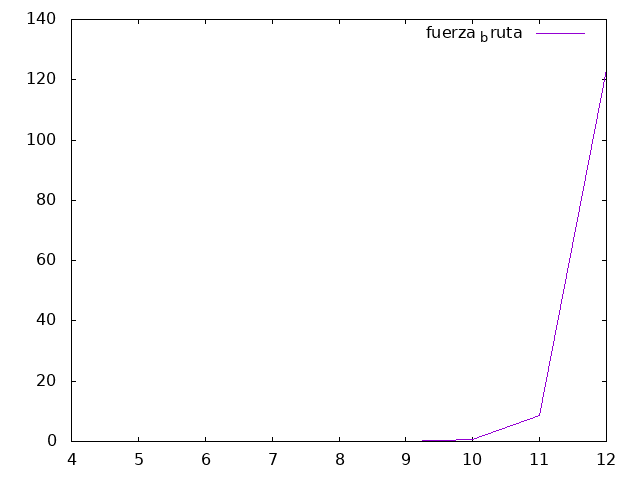
\includegraphics[width=0.8\textwidth]{./imagenes/fuerza_bruta}
		\caption{Fuerza bruta} \label{fig:1}
	\end{figure}
	
	Tras la ejecución del programa con backtraking se han obtenido los siguientes resultados, donde la primera columna es el tamaño y la segunda el tiempo: \\
	
	\lstset{language=C}
	\begin{lstlisting}[frame=single]
4 5.5e-06
5 6.7e-06
6 2.07e-05
7 7.99e-05
8 0.0003285
9 0.0016537
10 0.0081833
11 0.0413678
12 0.252748
13 1.48644
14 9.62347
15 66.6847
	\end{lstlisting} 

	La gráfica obtenida con las salidas de backtraking se muestra en la figura 4.2: \\

\begin{figure}[htb]
	\centering
	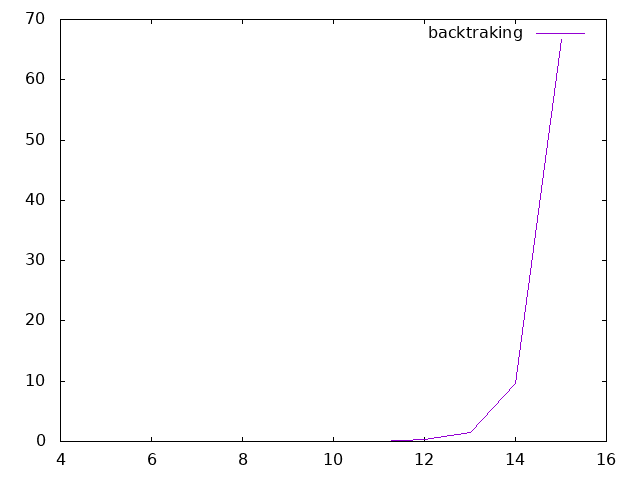
\includegraphics[width=0.8\textwidth]{./imagenes/backtraking}
	\caption{Fuerza bruta} \label{fig:1}
\end{figure}
	


	%-----------------------------------------------------------------------
	%							BIBLIOGRAFIA
	%-----------------------------------------------------------------------
	% Referencia a bibliografia			En \cite{Baz}
	% Referencia a figura				La figura (\ref{fig:1})
	% Espacio entre lineas				\vspace{0.06in}
	% Figura con comentario al pie
	%\begin{figure}[htb]
	%	\centering
	%	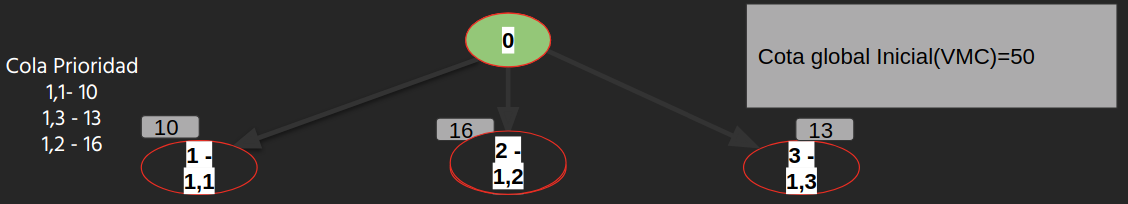
\includegraphics[width=0.4\textwidth]{./imagenes/1}
	%	\caption{Universidad de Granada.} \label{fig:1}
	%\end{figure}
	%\begin{thebibliography}{99}
	%	\bibitem{Baz} 
	%	\textsc{Bazaraa, M.S., J.J. Jarvis}
	%	\textit{Programacuib}.
	%	\newline
	%	\url{https://www.google.es}	
	%\end{thebibliography}

	


\end{document}